% Created by tikzDevice version 0.12.3 on 2020-01-28 12:23:04
% !TEX encoding = UTF-8 Unicode
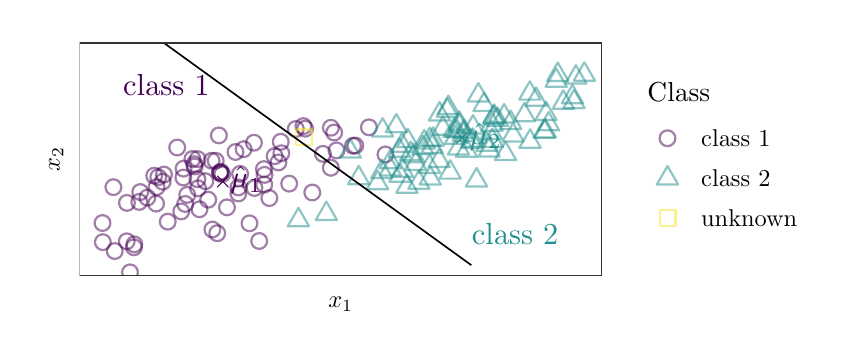
\begin{tikzpicture}[x=1pt,y=1pt]
\definecolor{fillColor}{RGB}{255,255,255}
\path[use as bounding box,fill=fillColor,fill opacity=0.00] (0,0) rectangle (289.08,108.41);
\begin{scope}
\path[clip] (  0.00,  0.00) rectangle (289.08,108.41);
\definecolor{drawColor}{RGB}{255,255,255}
\definecolor{fillColor}{RGB}{255,255,255}

\path[draw=drawColor,line width= 0.6pt,line join=round,line cap=round,fill=fillColor] (  0.00,  0.00) rectangle (289.08,108.41);
\end{scope}
\begin{scope}
\path[clip] ( 18.77, 18.77) rectangle (207.47,102.91);
\definecolor{fillColor}{RGB}{255,255,255}

\path[fill=fillColor] ( 18.77, 18.77) rectangle (207.47,102.91);
\definecolor{drawColor}{RGB}{68,1,84}

\path[draw=drawColor,draw opacity=0.50,line width= 0.8pt,line join=round,line cap=round] (100.26, 71.91) circle (  2.85);

\path[draw=drawColor,draw opacity=0.50,line width= 0.8pt,line join=round,line cap=round] ( 67.94, 60.32) circle (  2.85);

\path[draw=drawColor,draw opacity=0.50,line width= 0.8pt,line join=round,line cap=round] ( 27.04, 37.82) circle (  2.85);

\path[draw=drawColor,draw opacity=0.50,line width= 0.8pt,line join=round,line cap=round] ( 54.03, 65.11) circle (  2.85);

\path[draw=drawColor,draw opacity=0.50,line width= 0.8pt,line join=round,line cap=round] ( 62.08, 42.79) circle (  2.85);

\path[draw=drawColor,draw opacity=0.50,line width= 0.8pt,line join=round,line cap=round] ( 81.95, 50.47) circle (  2.85);

\path[draw=drawColor,draw opacity=0.50,line width= 0.8pt,line join=round,line cap=round] ( 64.19, 52.93) circle (  2.85);

\path[draw=drawColor,draw opacity=0.50,line width= 0.8pt,line join=round,line cap=round] ( 87.32, 46.84) circle (  2.85);

\path[draw=drawColor,draw opacity=0.50,line width= 0.8pt,line join=round,line cap=round] ( 48.78, 52.75) circle (  2.85);

\path[draw=drawColor,draw opacity=0.50,line width= 0.8pt,line join=round,line cap=round] (123.31, 72.40) circle (  2.85);

\path[draw=drawColor,draw opacity=0.50,line width= 0.8pt,line join=round,line cap=round] ( 96.88, 71.80) circle (  2.85);

\path[draw=drawColor,draw opacity=0.50,line width= 0.8pt,line join=round,line cap=round] ( 55.49, 42.01) circle (  2.85);

\path[draw=drawColor,draw opacity=0.50,line width= 0.8pt,line join=round,line cap=round] (102.85, 48.85) circle (  2.85);

\path[draw=drawColor,draw opacity=0.50,line width= 0.8pt,line join=round,line cap=round] ( 91.45, 67.17) circle (  2.85);

\path[draw=drawColor,draw opacity=0.50,line width= 0.8pt,line join=round,line cap=round] (106.69, 62.81) circle (  2.85);

\path[draw=drawColor,draw opacity=0.50,line width= 0.8pt,line join=round,line cap=round] ( 40.31, 45.45) circle (  2.85);

\path[draw=drawColor,draw opacity=0.50,line width= 0.8pt,line join=round,line cap=round] (129.28, 62.60) circle (  2.85);

\path[draw=drawColor,draw opacity=0.50,line width= 0.8pt,line join=round,line cap=round] ( 56.92, 44.71) circle (  2.85);

\path[draw=drawColor,draw opacity=0.50,line width= 0.8pt,line join=round,line cap=round] ( 85.49, 51.71) circle (  2.85);

\path[draw=drawColor,draw opacity=0.50,line width= 0.8pt,line join=round,line cap=round] ( 60.34, 58.27) circle (  2.85);

\path[draw=drawColor,draw opacity=0.50,line width= 0.8pt,line join=round,line cap=round] ( 38.38, 29.05) circle (  2.85);

\path[draw=drawColor,draw opacity=0.50,line width= 0.8pt,line join=round,line cap=round] ( 56.25, 54.26) circle (  2.85);

\path[draw=drawColor,draw opacity=0.50,line width= 0.8pt,line join=round,line cap=round] ( 31.47, 27.70) circle (  2.85);

\path[draw=drawColor,draw opacity=0.50,line width= 0.8pt,line join=round,line cap=round] ( 27.16, 30.91) circle (  2.85);

\path[draw=drawColor,draw opacity=0.50,line width= 0.8pt,line join=round,line cap=round] ( 59.54, 60.96) circle (  2.85);

\path[draw=drawColor,draw opacity=0.50,line width= 0.8pt,line join=round,line cap=round] ( 85.59, 55.22) circle (  2.85);

\path[draw=drawColor,draw opacity=0.50,line width= 0.8pt,line join=round,line cap=round] ( 69.09, 69.48) circle (  2.85);

\path[draw=drawColor,draw opacity=0.50,line width= 0.8pt,line join=round,line cap=round] ( 66.47, 60.31) circle (  2.85);

\path[draw=drawColor,draw opacity=0.50,line width= 0.8pt,line join=round,line cap=round] ( 40.67, 49.01) circle (  2.85);

\path[draw=drawColor,draw opacity=0.50,line width= 0.8pt,line join=round,line cap=round] ( 80.15, 37.71) circle (  2.85);

\path[draw=drawColor,draw opacity=0.50,line width= 0.8pt,line join=round,line cap=round] ( 89.24, 61.99) circle (  2.85);

\path[draw=drawColor,draw opacity=0.50,line width= 0.8pt,line join=round,line cap=round] (118.39, 65.82) circle (  2.85);

\path[draw=drawColor,draw opacity=0.50,line width= 0.8pt,line join=round,line cap=round] ( 78.04, 64.50) circle (  2.85);

\path[draw=drawColor,draw opacity=0.50,line width= 0.8pt,line join=round,line cap=round] ( 60.21, 59.09) circle (  2.85);

\path[draw=drawColor,draw opacity=0.50,line width= 0.8pt,line join=round,line cap=round] ( 76.15, 50.67) circle (  2.85);

\path[draw=drawColor,draw opacity=0.50,line width= 0.8pt,line join=round,line cap=round] (110.74, 70.52) circle (  2.85);

\path[draw=drawColor,draw opacity=0.50,line width= 0.8pt,line join=round,line cap=round] ( 36.98, 19.98) circle (  2.85);

\path[draw=drawColor,draw opacity=0.50,line width= 0.8pt,line join=round,line cap=round] ( 81.76, 66.83) circle (  2.85);

\path[draw=drawColor,draw opacity=0.50,line width= 0.8pt,line join=round,line cap=round] ( 49.24, 55.33) circle (  2.85);

\path[draw=drawColor,draw opacity=0.50,line width= 0.8pt,line join=round,line cap=round] ( 66.74, 35.47) circle (  2.85);

\path[draw=drawColor,draw opacity=0.50,line width= 0.8pt,line join=round,line cap=round] (109.55, 57.78) circle (  2.85);

\path[draw=drawColor,draw opacity=0.50,line width= 0.8pt,line join=round,line cap=round] ( 35.87, 45.09) circle (  2.85);

\path[draw=drawColor,draw opacity=0.50,line width= 0.8pt,line join=round,line cap=round] ( 61.39, 60.91) circle (  2.85);

\path[draw=drawColor,draw opacity=0.50,line width= 0.8pt,line join=round,line cap=round] ( 69.72, 56.36) circle (  2.85);

\path[draw=drawColor,draw opacity=0.50,line width= 0.8pt,line join=round,line cap=round] ( 70.32, 55.49) circle (  2.85);

\path[draw=drawColor,draw opacity=0.50,line width= 0.8pt,line join=round,line cap=round] ( 38.54, 30.13) circle (  2.85);

\path[draw=drawColor,draw opacity=0.50,line width= 0.8pt,line join=round,line cap=round] ( 69.62, 56.00) circle (  2.85);

\path[draw=drawColor,draw opacity=0.50,line width= 0.8pt,line join=round,line cap=round] ( 65.22, 46.25) circle (  2.85);

\path[draw=drawColor,draw opacity=0.50,line width= 0.8pt,line join=round,line cap=round] ( 30.97, 50.78) circle (  2.85);

\path[draw=drawColor,draw opacity=0.50,line width= 0.8pt,line join=round,line cap=round] ( 50.61, 38.31) circle (  2.85);

\path[draw=drawColor,draw opacity=0.50,line width= 0.8pt,line join=round,line cap=round] ( 83.66, 31.33) circle (  2.85);

\path[draw=drawColor,draw opacity=0.50,line width= 0.8pt,line join=round,line cap=round] ( 46.41, 44.84) circle (  2.85);

\path[draw=drawColor,draw opacity=0.50,line width= 0.8pt,line join=round,line cap=round] (111.58, 64.05) circle (  2.85);

\path[draw=drawColor,draw opacity=0.50,line width= 0.8pt,line join=round,line cap=round] ( 75.09, 63.49) circle (  2.85);

\path[draw=drawColor,draw opacity=0.50,line width= 0.8pt,line join=round,line cap=round] ( 94.50, 52.05) circle (  2.85);

\path[draw=drawColor,draw opacity=0.50,line width= 0.8pt,line join=round,line cap=round] (109.57, 72.24) circle (  2.85);

\path[draw=drawColor,draw opacity=0.50,line width= 0.8pt,line join=round,line cap=round] ( 99.62, 72.84) circle (  2.85);

\path[draw=drawColor,draw opacity=0.50,line width= 0.8pt,line join=round,line cap=round] ( 91.66, 63.04) circle (  2.85);

\path[draw=drawColor,draw opacity=0.50,line width= 0.8pt,line join=round,line cap=round] ( 68.50, 34.14) circle (  2.85);

\path[draw=drawColor,draw opacity=0.50,line width= 0.8pt,line join=round,line cap=round] (117.55, 65.72) circle (  2.85);

\path[draw=drawColor,draw opacity=0.50,line width= 0.8pt,line join=round,line cap=round] ( 76.12, 48.49) circle (  2.85);

\path[draw=drawColor,draw opacity=0.50,line width= 0.8pt,line join=round,line cap=round] ( 45.71, 54.92) circle (  2.85);

\path[draw=drawColor,draw opacity=0.50,line width= 0.8pt,line join=round,line cap=round] ( 76.76, 55.57) circle (  2.85);

\path[draw=drawColor,draw opacity=0.50,line width= 0.8pt,line join=round,line cap=round] ( 56.33, 57.47) circle (  2.85);

\path[draw=drawColor,draw opacity=0.50,line width= 0.8pt,line join=round,line cap=round] ( 57.66, 48.00) circle (  2.85);

\path[draw=drawColor,draw opacity=0.50,line width= 0.8pt,line join=round,line cap=round] ( 90.60, 59.70) circle (  2.85);

\path[draw=drawColor,draw opacity=0.50,line width= 0.8pt,line join=round,line cap=round] ( 46.59, 50.78) circle (  2.85);

\path[draw=drawColor,draw opacity=0.50,line width= 0.8pt,line join=round,line cap=round] ( 72.01, 43.49) circle (  2.85);

\path[draw=drawColor,draw opacity=0.50,line width= 0.8pt,line join=round,line cap=round] ( 47.18, 54.39) circle (  2.85);

\path[draw=drawColor,draw opacity=0.50,line width= 0.8pt,line join=round,line cap=round] ( 43.25, 46.99) circle (  2.85);

\path[draw=drawColor,draw opacity=0.50,line width= 0.8pt,line join=round,line cap=round] ( 69.48, 55.89) circle (  2.85);

\path[draw=drawColor,draw opacity=0.50,line width= 0.8pt,line join=round,line cap=round] ( 61.32, 53.67) circle (  2.85);

\path[draw=drawColor,draw opacity=0.50,line width= 0.8pt,line join=round,line cap=round] ( 61.56, 50.35) circle (  2.85);

\path[draw=drawColor,draw opacity=0.50,line width= 0.8pt,line join=round,line cap=round] ( 85.37, 57.29) circle (  2.85);

\path[draw=drawColor,draw opacity=0.50,line width= 0.8pt,line join=round,line cap=round] ( 35.80, 31.22) circle (  2.85);
\definecolor{drawColor}{RGB}{33,143,141}

\path[draw=drawColor,draw opacity=0.50,line width= 0.8pt,line join=round,line cap=round] (148.70, 64.70) --
	(152.54, 58.05) --
	(144.85, 58.05) --
	(148.70, 64.70);

\path[draw=drawColor,draw opacity=0.50,line width= 0.8pt,line join=round,line cap=round] (183.74, 86.82) --
	(187.59, 80.17) --
	(179.90, 80.17) --
	(183.74, 86.82);

\path[draw=drawColor,draw opacity=0.50,line width= 0.8pt,line join=round,line cap=round] (169.77, 79.57) --
	(173.61, 72.92) --
	(165.92, 72.92) --
	(169.77, 79.57);

\path[draw=drawColor,draw opacity=0.50,line width= 0.8pt,line join=round,line cap=round] (172.66, 67.25) --
	(176.51, 60.60) --
	(168.82, 60.60) --
	(172.66, 67.25);

\path[draw=drawColor,draw opacity=0.50,line width= 0.8pt,line join=round,line cap=round] (127.97, 60.74) --
	(131.81, 54.08) --
	(124.13, 54.08) --
	(127.97, 60.74);

\path[draw=drawColor,draw opacity=0.50,line width= 0.8pt,line join=round,line cap=round] (155.96, 78.20) --
	(159.80, 71.54) --
	(152.11, 71.54) --
	(155.96, 78.20);

\path[draw=drawColor,draw opacity=0.50,line width= 0.8pt,line join=round,line cap=round] (135.48, 61.16) --
	(139.33, 54.51) --
	(131.64, 54.51) --
	(135.48, 61.16);

\path[draw=drawColor,draw opacity=0.50,line width= 0.8pt,line join=round,line cap=round] (116.60, 68.11) --
	(120.44, 61.46) --
	(112.76, 61.46) --
	(116.60, 68.11);

\path[draw=drawColor,draw opacity=0.50,line width= 0.8pt,line join=round,line cap=round] (201.16, 95.91) --
	(205.00, 89.26) --
	(197.32, 89.26) --
	(201.16, 95.91);

\path[draw=drawColor,draw opacity=0.50,line width= 0.8pt,line join=round,line cap=round] (119.62, 58.46) --
	(123.46, 51.80) --
	(115.77, 51.80) --
	(119.62, 58.46);

\path[draw=drawColor,draw opacity=0.50,line width= 0.8pt,line join=round,line cap=round] (131.00, 64.24) --
	(134.84, 57.58) --
	(127.16, 57.58) --
	(131.00, 64.24);

\path[draw=drawColor,draw opacity=0.50,line width= 0.8pt,line join=round,line cap=round] (134.37, 68.42) --
	(138.22, 61.77) --
	(130.53, 61.77) --
	(134.37, 68.42);

\path[draw=drawColor,draw opacity=0.50,line width= 0.8pt,line join=round,line cap=round] (138.44, 67.23) --
	(142.28, 60.57) --
	(134.60, 60.57) --
	(138.44, 67.23);

\path[draw=drawColor,draw opacity=0.50,line width= 0.8pt,line join=round,line cap=round] (134.53, 59.43) --
	(138.37, 52.77) --
	(130.68, 52.77) --
	(134.53, 59.43);

\path[draw=drawColor,draw opacity=0.50,line width= 0.8pt,line join=round,line cap=round] (145.32, 72.33) --
	(149.16, 65.68) --
	(141.47, 65.68) --
	(145.32, 72.33);

\path[draw=drawColor,draw opacity=0.50,line width= 0.8pt,line join=round,line cap=round] (131.06, 61.68) --
	(134.90, 55.02) --
	(127.22, 55.02) --
	(131.06, 61.68);

\path[draw=drawColor,draw opacity=0.50,line width= 0.8pt,line join=round,line cap=round] (181.45, 89.06) --
	(185.29, 82.41) --
	(177.61, 82.41) --
	(181.45, 89.06);

\path[draw=drawColor,draw opacity=0.50,line width= 0.8pt,line join=round,line cap=round] (150.02, 76.35) --
	(153.87, 69.70) --
	(146.18, 69.70) --
	(150.02, 76.35);

\path[draw=drawColor,draw opacity=0.50,line width= 0.8pt,line join=round,line cap=round] (164.90, 84.96) --
	(168.75, 78.30) --
	(161.06, 78.30) --
	(164.90, 84.96);

\path[draw=drawColor,draw opacity=0.50,line width= 0.8pt,line join=round,line cap=round] (126.43, 56.71) --
	(130.27, 50.06) --
	(122.59, 50.06) --
	(126.43, 56.71);

\path[draw=drawColor,draw opacity=0.50,line width= 0.8pt,line join=round,line cap=round] (160.35, 71.67) --
	(164.19, 65.02) --
	(156.51, 65.02) --
	(160.35, 71.67);

\path[draw=drawColor,draw opacity=0.50,line width= 0.8pt,line join=round,line cap=round] (151.67, 82.91) --
	(155.51, 76.25) --
	(147.82, 76.25) --
	(151.67, 82.91);

\path[draw=drawColor,draw opacity=0.50,line width= 0.8pt,line join=round,line cap=round] (157.45, 74.20) --
	(161.29, 67.55) --
	(153.61, 67.55) --
	(157.45, 74.20);

\path[draw=drawColor,draw opacity=0.50,line width= 0.8pt,line join=round,line cap=round] (160.87, 72.08) --
	(164.72, 65.42) --
	(157.03, 65.42) --
	(160.87, 72.08);

\path[draw=drawColor,draw opacity=0.50,line width= 0.8pt,line join=round,line cap=round] (145.47, 58.38) --
	(149.31, 51.72) --
	(141.63, 51.72) --
	(145.47, 58.38);

\path[draw=drawColor,draw opacity=0.50,line width= 0.8pt,line join=round,line cap=round] (139.51, 66.44) --
	(143.35, 59.78) --
	(135.67, 59.78) --
	(139.51, 66.44);

\path[draw=drawColor,draw opacity=0.50,line width= 0.8pt,line join=round,line cap=round] (142.84, 69.34) --
	(146.68, 62.68) --
	(138.99, 62.68) --
	(142.84, 69.34);

\path[draw=drawColor,draw opacity=0.50,line width= 0.8pt,line join=round,line cap=round] (152.66, 60.51) --
	(156.50, 53.86) --
	(148.81, 53.86) --
	(152.66, 60.51);

\path[draw=drawColor,draw opacity=0.50,line width= 0.8pt,line join=round,line cap=round] (188.24, 77.96) --
	(192.08, 71.31) --
	(184.40, 71.31) --
	(188.24, 77.96);

\path[draw=drawColor,draw opacity=0.50,line width= 0.8pt,line join=round,line cap=round] (190.97, 93.70) --
	(194.81, 87.05) --
	(187.12, 87.05) --
	(190.97, 93.70);

\path[draw=drawColor,draw opacity=0.50,line width= 0.8pt,line join=round,line cap=round] (193.56, 85.79) --
	(197.40, 79.13) --
	(189.72, 79.13) --
	(193.56, 85.79);

\path[draw=drawColor,draw opacity=0.50,line width= 0.8pt,line join=round,line cap=round] (148.83, 81.55) --
	(152.67, 74.90) --
	(144.99, 74.90) --
	(148.83, 81.55);

\path[draw=drawColor,draw opacity=0.50,line width= 0.8pt,line join=round,line cap=round] (166.73, 68.48) --
	(170.58, 61.82) --
	(162.89, 61.82) --
	(166.73, 68.48);

\path[draw=drawColor,draw opacity=0.50,line width= 0.8pt,line join=round,line cap=round] (186.67, 75.24) --
	(190.51, 68.59) --
	(182.83, 68.59) --
	(186.67, 75.24);

\path[draw=drawColor,draw opacity=0.50,line width= 0.8pt,line join=round,line cap=round] (140.19, 63.65) --
	(144.03, 56.99) --
	(136.35, 56.99) --
	(140.19, 63.65);

\path[draw=drawColor,draw opacity=0.50,line width= 0.8pt,line join=round,line cap=round] (156.01, 77.28) --
	(159.86, 70.62) --
	(152.17, 70.62) --
	(156.01, 77.28);

\path[draw=drawColor,draw opacity=0.50,line width= 0.8pt,line join=round,line cap=round] (157.65, 75.28) --
	(161.49, 68.62) --
	(153.81, 68.62) --
	(157.65, 75.28);

\path[draw=drawColor,draw opacity=0.50,line width= 0.8pt,line join=round,line cap=round] (107.93, 45.58) --
	(111.77, 38.92) --
	(104.09, 38.92) --
	(107.93, 45.58);

\path[draw=drawColor,draw opacity=0.50,line width= 0.8pt,line join=round,line cap=round] (191.54, 95.82) --
	(195.38, 89.17) --
	(187.69, 89.17) --
	(191.54, 95.82);

\path[draw=drawColor,draw opacity=0.50,line width= 0.8pt,line join=round,line cap=round] (137.07, 55.45) --
	(140.91, 48.79) --
	(133.22, 48.79) --
	(137.07, 55.45);

\path[draw=drawColor,draw opacity=0.50,line width= 0.8pt,line join=round,line cap=round] ( 97.85, 43.31) --
	(101.69, 36.66) --
	( 94.00, 36.66) --
	( 97.85, 43.31);

\path[draw=drawColor,draw opacity=0.50,line width= 0.8pt,line join=round,line cap=round] (165.96, 70.60) --
	(169.80, 63.94) --
	(162.12, 63.94) --
	(165.96, 70.60);

\path[draw=drawColor,draw opacity=0.50,line width= 0.8pt,line join=round,line cap=round] (167.88, 71.92) --
	(171.73, 65.26) --
	(164.04, 65.26) --
	(167.88, 71.92);

\path[draw=drawColor,draw opacity=0.50,line width= 0.8pt,line join=round,line cap=round] (154.57, 73.13) --
	(158.41, 66.47) --
	(150.72, 66.47) --
	(154.57, 73.13);

\path[draw=drawColor,draw opacity=0.50,line width= 0.8pt,line join=round,line cap=round] (154.06, 75.69) --
	(157.91, 69.03) --
	(150.22, 69.03) --
	(154.06, 75.69);

\path[draw=drawColor,draw opacity=0.50,line width= 0.8pt,line join=round,line cap=round] (141.37, 56.86) --
	(145.21, 50.20) --
	(137.52, 50.20) --
	(141.37, 56.86);

\path[draw=drawColor,draw opacity=0.50,line width= 0.8pt,line join=round,line cap=round] (187.04, 75.43) --
	(190.89, 68.77) --
	(183.20, 68.77) --
	(187.04, 75.43);

\path[draw=drawColor,draw opacity=0.50,line width= 0.8pt,line join=round,line cap=round] (197.42, 85.97) --
	(201.27, 79.31) --
	(193.58, 79.31) --
	(197.42, 85.97);

\path[draw=drawColor,draw opacity=0.50,line width= 0.8pt,line join=round,line cap=round] (162.19, 57.69) --
	(166.03, 51.04) --
	(158.34, 51.04) --
	(162.19, 57.69);

\path[draw=drawColor,draw opacity=0.50,line width= 0.8pt,line join=round,line cap=round] (160.93, 76.81) --
	(164.77, 70.15) --
	(157.08, 70.15) --
	(160.93, 76.81);

\path[draw=drawColor,draw opacity=0.50,line width= 0.8pt,line join=round,line cap=round] (143.30, 71.43) --
	(147.15, 64.78) --
	(139.46, 64.78) --
	(143.30, 71.43);

\path[draw=drawColor,draw opacity=0.50,line width= 0.8pt,line join=round,line cap=round] (133.21, 77.24) --
	(137.05, 70.59) --
	(129.36, 70.59) --
	(133.21, 77.24);

\path[draw=drawColor,draw opacity=0.50,line width= 0.8pt,line join=round,line cap=round] (187.30, 81.67) --
	(191.14, 75.01) --
	(183.46, 75.01) --
	(187.30, 81.67);

\path[draw=drawColor,draw opacity=0.50,line width= 0.8pt,line join=round,line cap=round] (167.52, 74.81) --
	(171.36, 68.15) --
	(163.68, 68.15) --
	(167.52, 74.81);

\path[draw=drawColor,draw opacity=0.50,line width= 0.8pt,line join=round,line cap=round] (198.10, 94.87) --
	(201.94, 88.21) --
	(194.26, 88.21) --
	(198.10, 94.87);

\path[draw=drawColor,draw opacity=0.50,line width= 0.8pt,line join=round,line cap=round] (146.15, 69.76) --
	(150.00, 63.10) --
	(142.31, 63.10) --
	(146.15, 69.76);

\path[draw=drawColor,draw opacity=0.50,line width= 0.8pt,line join=round,line cap=round] (196.84, 87.77) --
	(200.68, 81.11) --
	(193.00, 81.11) --
	(196.84, 87.77);

\path[draw=drawColor,draw opacity=0.50,line width= 0.8pt,line join=round,line cap=round] (135.29, 70.27) --
	(139.13, 63.61) --
	(131.45, 63.61) --
	(135.29, 70.27);

\path[draw=drawColor,draw opacity=0.50,line width= 0.8pt,line join=round,line cap=round] (155.66, 69.20) --
	(159.50, 62.55) --
	(151.82, 62.55) --
	(155.66, 69.20);

\path[draw=drawColor,draw opacity=0.50,line width= 0.8pt,line join=round,line cap=round] (137.34, 71.90) --
	(141.18, 65.25) --
	(133.49, 65.25) --
	(137.34, 71.90);

\path[draw=drawColor,draw opacity=0.50,line width= 0.8pt,line join=round,line cap=round] (181.55, 71.70) --
	(185.39, 65.04) --
	(177.70, 65.04) --
	(181.55, 71.70);

\path[draw=drawColor,draw opacity=0.50,line width= 0.8pt,line join=round,line cap=round] (167.80, 77.84) --
	(171.64, 71.19) --
	(163.96, 71.19) --
	(167.80, 77.84);

\path[draw=drawColor,draw opacity=0.50,line width= 0.8pt,line join=round,line cap=round] (154.95, 75.56) --
	(158.79, 68.90) --
	(151.10, 68.90) --
	(154.95, 75.56);

\path[draw=drawColor,draw opacity=0.50,line width= 0.8pt,line join=round,line cap=round] (174.54, 78.46) --
	(178.39, 71.80) --
	(170.70, 71.80) --
	(174.54, 78.46);

\path[draw=drawColor,draw opacity=0.50,line width= 0.8pt,line join=round,line cap=round] (145.21, 62.58) --
	(149.06, 55.93) --
	(141.37, 55.93) --
	(145.21, 62.58);

\path[draw=drawColor,draw opacity=0.50,line width= 0.8pt,line join=round,line cap=round] (158.58, 68.40) --
	(162.42, 61.74) --
	(154.74, 61.74) --
	(158.58, 68.40);

\path[draw=drawColor,draw opacity=0.50,line width= 0.8pt,line join=round,line cap=round] (168.55, 80.72) --
	(172.39, 74.07) --
	(164.70, 74.07) --
	(168.55, 80.72);

\path[draw=drawColor,draw opacity=0.50,line width= 0.8pt,line join=round,line cap=round] (162.86, 88.40) --
	(166.70, 81.74) --
	(159.01, 81.74) --
	(162.86, 88.40);

\path[draw=drawColor,draw opacity=0.50,line width= 0.8pt,line join=round,line cap=round] (175.39, 73.97) --
	(179.23, 67.31) --
	(171.54, 67.31) --
	(175.39, 73.97);

\path[draw=drawColor,draw opacity=0.50,line width= 0.8pt,line join=round,line cap=round] (172.17, 80.82) --
	(176.01, 74.16) --
	(168.33, 74.16) --
	(172.17, 80.82);

\path[draw=drawColor,draw opacity=0.50,line width= 0.8pt,line join=round,line cap=round] (179.51, 81.25) --
	(183.35, 74.60) --
	(175.67, 74.60) --
	(179.51, 81.25);

\path[draw=drawColor,draw opacity=0.50,line width= 0.8pt,line join=round,line cap=round] (152.00, 83.88) --
	(155.84, 77.22) --
	(148.16, 77.22) --
	(152.00, 83.88);

\path[draw=drawColor,draw opacity=0.50,line width= 0.8pt,line join=round,line cap=round] (128.26, 75.72) --
	(132.11, 69.06) --
	(124.42, 69.06) --
	(128.26, 75.72);

\path[draw=drawColor,draw opacity=0.50,line width= 0.8pt,line join=round,line cap=round] (146.56, 72.43) --
	(150.40, 65.77) --
	(142.72, 65.77) --
	(146.56, 72.43);

\path[draw=drawColor,draw opacity=0.50,line width= 0.8pt,line join=round,line cap=round] (168.35, 80.27) --
	(172.19, 73.62) --
	(164.51, 73.62) --
	(168.35, 80.27);
\definecolor{drawColor}{RGB}{247,230,32}

\path[draw=drawColor,draw opacity=0.50,line width= 0.8pt,line join=round,line cap=round] ( 96.91, 65.91) rectangle (102.62, 71.62);
\definecolor{drawColor}{RGB}{68,1,84}

\path[draw=drawColor,line width= 0.4pt,line join=round,line cap=round] ( 68.58, 50.87) -- ( 72.50, 54.80);

\path[draw=drawColor,line width= 0.4pt,line join=round,line cap=round] ( 68.58, 54.80) -- ( 72.50, 50.87);
\definecolor{drawColor}{RGB}{33,143,141}

\path[draw=drawColor,line width= 0.4pt,line join=round,line cap=round] (154.99, 66.68) -- (158.92, 70.60);

\path[draw=drawColor,line width= 0.4pt,line join=round,line cap=round] (154.99, 70.60) -- (158.92, 66.68);
\definecolor{drawColor}{RGB}{68,1,84}

\node[text=drawColor,anchor=base,inner sep=0pt, outer sep=0pt, scale=  1.10] at ( 79.12, 50.56) {$\hat{\mu}_1$};
\definecolor{drawColor}{RGB}{33,143,141}

\node[text=drawColor,anchor=base,inner sep=0pt, outer sep=0pt, scale=  1.10] at (165.53, 66.37) {$\hat{\mu}_2$};
\definecolor{drawColor}{RGB}{0,0,0}

\path[draw=drawColor,line width= 0.6pt,line join=round] ( 41.61,108.41) --
	(160.30, 22.60);
\definecolor{drawColor}{RGB}{68,1,84}

\node[text=drawColor,anchor=base west,inner sep=0pt, outer sep=0pt, scale=  1.10] at ( 34.47, 83.90) {class 1};
\definecolor{drawColor}{RGB}{33,143,141}

\node[text=drawColor,anchor=base east,inner sep=0pt, outer sep=0pt, scale=  1.10] at (191.78, 30.18) {class 2};
\definecolor{drawColor}{gray}{0.20}

\path[draw=drawColor,line width= 0.6pt,line join=round,line cap=round] ( 18.77, 18.77) rectangle (207.47,102.91);
\end{scope}
\begin{scope}
\path[clip] (  0.00,  0.00) rectangle (289.08,108.41);
\definecolor{drawColor}{RGB}{0,0,0}

\node[text=drawColor,anchor=base,inner sep=0pt, outer sep=0pt, scale=  0.88] at (113.12,  7.21) {$x_1$};
\end{scope}
\begin{scope}
\path[clip] (  0.00,  0.00) rectangle (289.08,108.41);
\definecolor{drawColor}{RGB}{0,0,0}

\node[text=drawColor,rotate= 90.00,anchor=base,inner sep=0pt, outer sep=0pt, scale=  0.88] at ( 11.56, 60.84) {$x_2$};
\end{scope}
\begin{scope}
\path[clip] (  0.00,  0.00) rectangle (289.08,108.41);
\definecolor{fillColor}{RGB}{255,255,255}

\path[fill=fillColor] (218.47, 26.81) rectangle (283.58, 94.87);
\end{scope}
\begin{scope}
\path[clip] (  0.00,  0.00) rectangle (289.08,108.41);
\definecolor{drawColor}{RGB}{0,0,0}

\node[text=drawColor,anchor=base west,inner sep=0pt, outer sep=0pt, scale=  0.99] at (223.97, 81.59) {Class};
\end{scope}
\begin{scope}
\path[clip] (  0.00,  0.00) rectangle (289.08,108.41);
\definecolor{fillColor}{RGB}{255,255,255}

\path[fill=fillColor] (223.97, 61.22) rectangle (238.43, 75.67);
\end{scope}
\begin{scope}
\path[clip] (  0.00,  0.00) rectangle (289.08,108.41);
\definecolor{drawColor}{RGB}{68,1,84}

\path[draw=drawColor,draw opacity=0.50,line width= 0.8pt,line join=round,line cap=round] (231.20, 68.45) circle (  2.85);
\end{scope}
\begin{scope}
\path[clip] (  0.00,  0.00) rectangle (289.08,108.41);
\definecolor{fillColor}{RGB}{255,255,255}

\path[fill=fillColor] (223.97, 46.76) rectangle (238.43, 61.22);
\end{scope}
\begin{scope}
\path[clip] (  0.00,  0.00) rectangle (289.08,108.41);
\definecolor{drawColor}{RGB}{33,143,141}

\path[draw=drawColor,draw opacity=0.50,line width= 0.8pt,line join=round,line cap=round] (231.20, 58.43) --
	(235.04, 51.77) --
	(227.36, 51.77) --
	(231.20, 58.43);
\end{scope}
\begin{scope}
\path[clip] (  0.00,  0.00) rectangle (289.08,108.41);
\definecolor{fillColor}{RGB}{255,255,255}

\path[fill=fillColor] (223.97, 32.31) rectangle (238.43, 46.76);
\end{scope}
\begin{scope}
\path[clip] (  0.00,  0.00) rectangle (289.08,108.41);
\definecolor{drawColor}{RGB}{247,230,32}

\path[draw=drawColor,draw opacity=0.50,line width= 0.8pt,line join=round,line cap=round] (228.35, 36.68) rectangle (234.05, 42.39);
\end{scope}
\begin{scope}
\path[clip] (  0.00,  0.00) rectangle (289.08,108.41);
\definecolor{drawColor}{RGB}{0,0,0}

\node[text=drawColor,anchor=base west,inner sep=0pt, outer sep=0pt, scale=  0.88] at (243.38, 65.42) {class 1};
\end{scope}
\begin{scope}
\path[clip] (  0.00,  0.00) rectangle (289.08,108.41);
\definecolor{drawColor}{RGB}{0,0,0}

\node[text=drawColor,anchor=base west,inner sep=0pt, outer sep=0pt, scale=  0.88] at (243.38, 50.96) {class 2};
\end{scope}
\begin{scope}
\path[clip] (  0.00,  0.00) rectangle (289.08,108.41);
\definecolor{drawColor}{RGB}{0,0,0}

\node[text=drawColor,anchor=base west,inner sep=0pt, outer sep=0pt, scale=  0.88] at (243.38, 36.51) {unknown};
\end{scope}
\end{tikzpicture}
